\documentclass[12pt, letterpaper]{article}
\usepackage[utf8]{inputenc}
\usepackage{amsfonts, amsmath, amssymb}
\makeatletter
\makeatother
\usepackage[hidelinks]{hyperref}
\usepackage{comment}
\usepackage{fullpage}
\usepackage[english]{babel}
\usepackage{pdfpages}
\usepackage{tikz}
\usepackage{graphicx}
\usepackage[colorinlistoftodos]{todonotes}
\usepackage[linesnumbered]{algorithm2e}
\usepackage{tabularx}
\usepackage{url}
\usepackage{hyperref}
\hypersetup{colorlinks=true}
\usepackage{multirow}
\usepackage[margin=0.5in]{geometry}
\usepackage[english]{babel}
\usepackage{mathtools}
\usepackage{booktabs}
\usepackage{physics}
\usepackage{enumitem}

\usepackage[thmmarks, thref]{ntheorem}

\theoremstyle{nonumberplain}
\theorembodyfont{\upshape}
\theoremseparator{.}
\theoremsymbol{\ensuremath{\square}}
\theoremsymbol{\ensuremath{\blacksquare}}
\newtheorem{sol}{Solution}
\theoremseparator{. ---}
\theoremsymbol{\mbox{\texttt{;o)}}}
\newtheorem{varsol}{Solution (variant)}

\DeclarePairedDelimiter\ceil{\lceil}{\rceil}
\DeclarePairedDelimiter\floor{\lfloor}{\rfloor}

\usetikzlibrary{matrix}
\setlength{\marginparwidth}{2cm} 

\title{MATH 4640 Numerical Analysis - HW 3 Solutions}

\author{Austin Barton}

\begin{document}
\maketitle

\vspace{2em}

\hspace{18pt}\textbf{Problem 1:} \medskip
Please see attached PDF with all written solutions for questions 1-5 and 7-8.

\hspace{18pt}\textbf{Problem 2:} \medskip
This problem accompanies the attached PDF which has a dedicated section for question 2. With the code in the following screenshots are the outputs for the code.

\begin{figure}[!htbp]
	\centering
	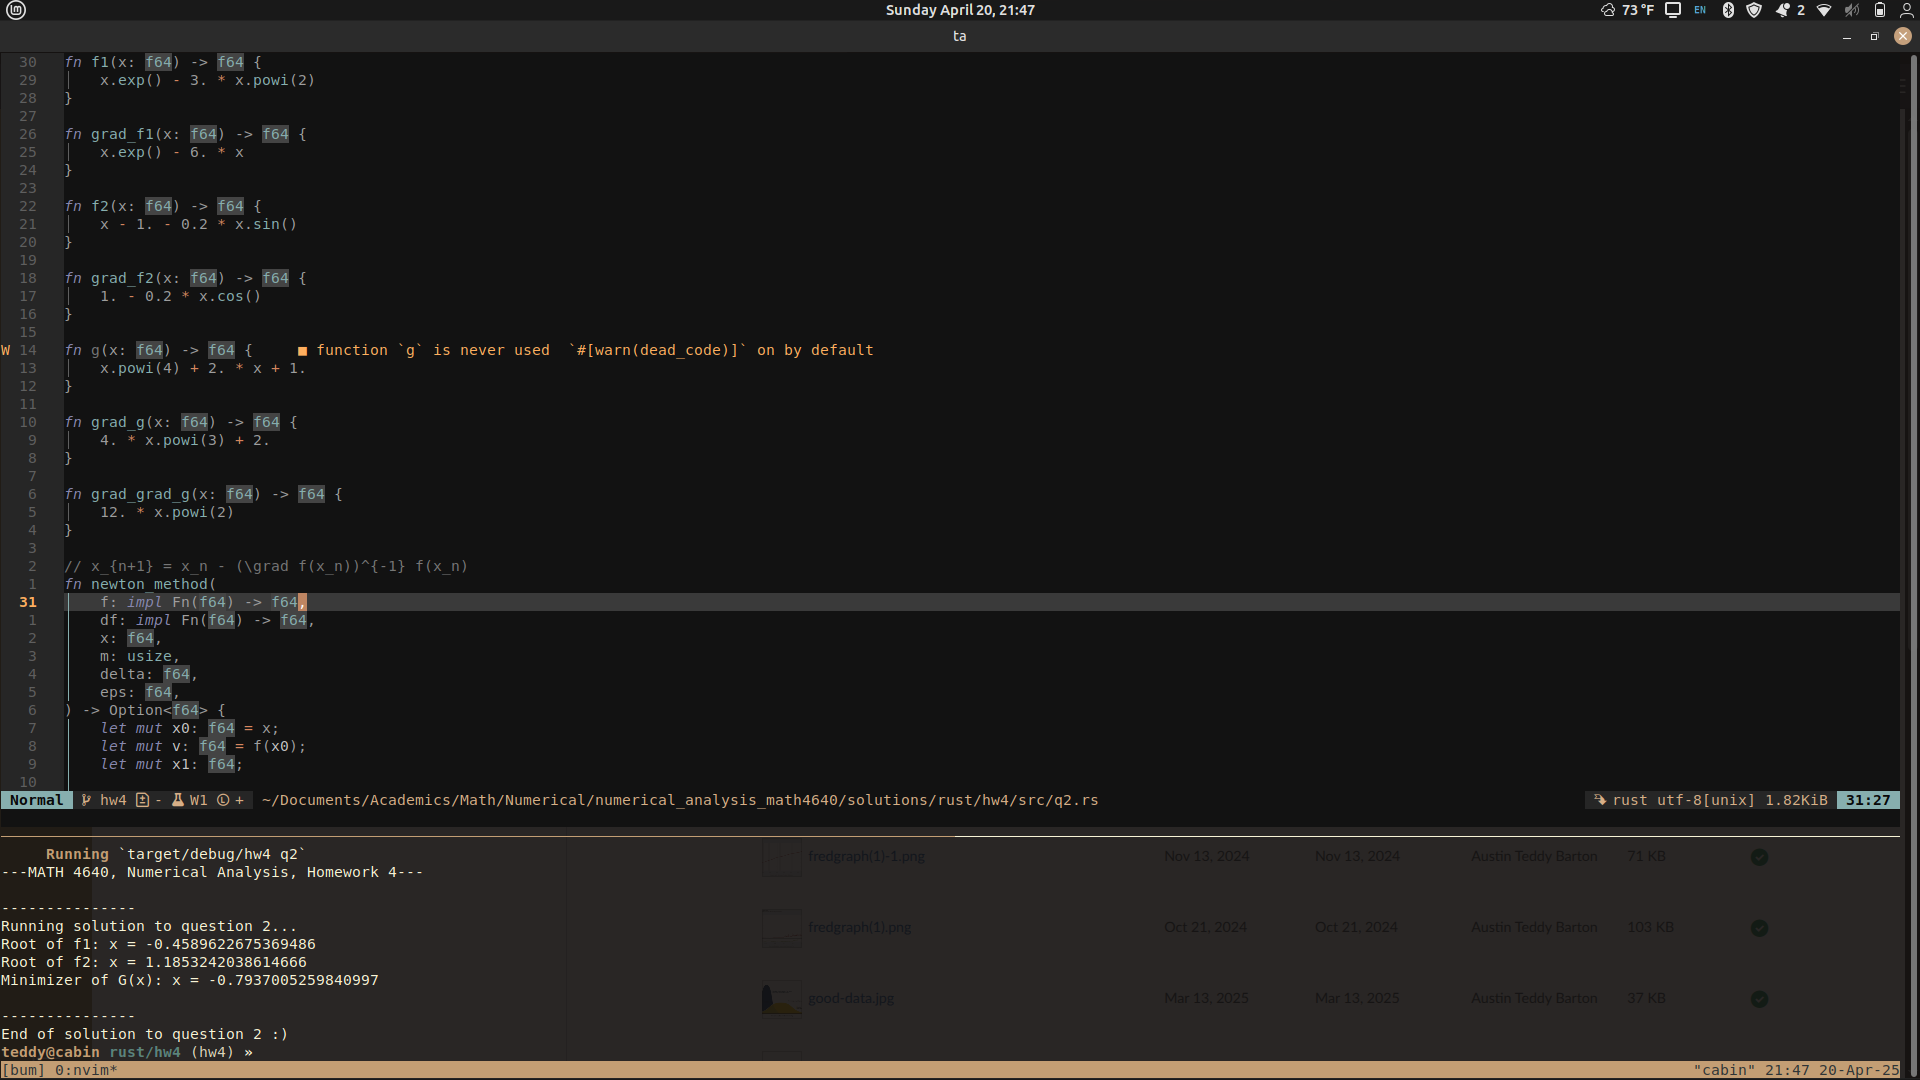
\includegraphics[width=0.8\textwidth]{numhw4q2-1.png}
\end{figure}
\begin{figure}[!htbp]
	\centering
	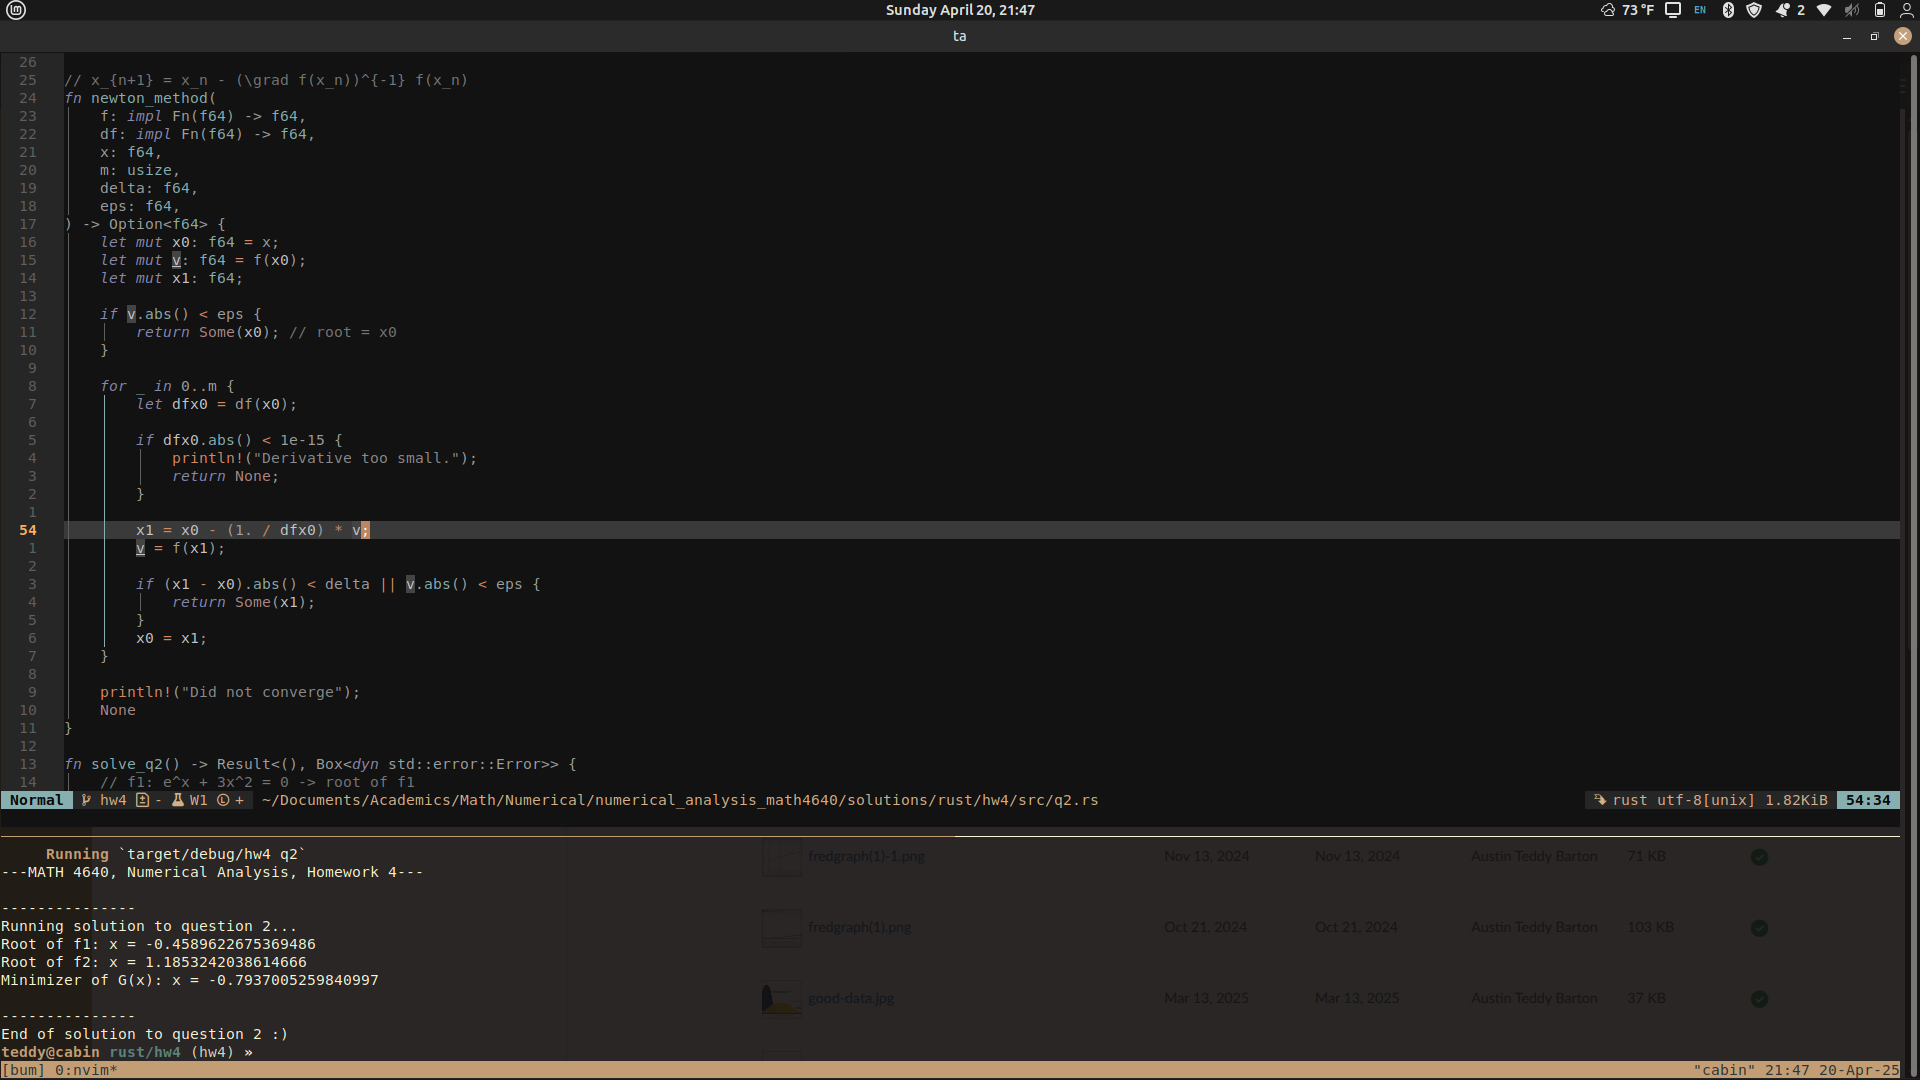
\includegraphics[width=0.8\textwidth]{numhw4q2-2.png}
\end{figure}
\begin{figure}[!htbp]
	\centering
	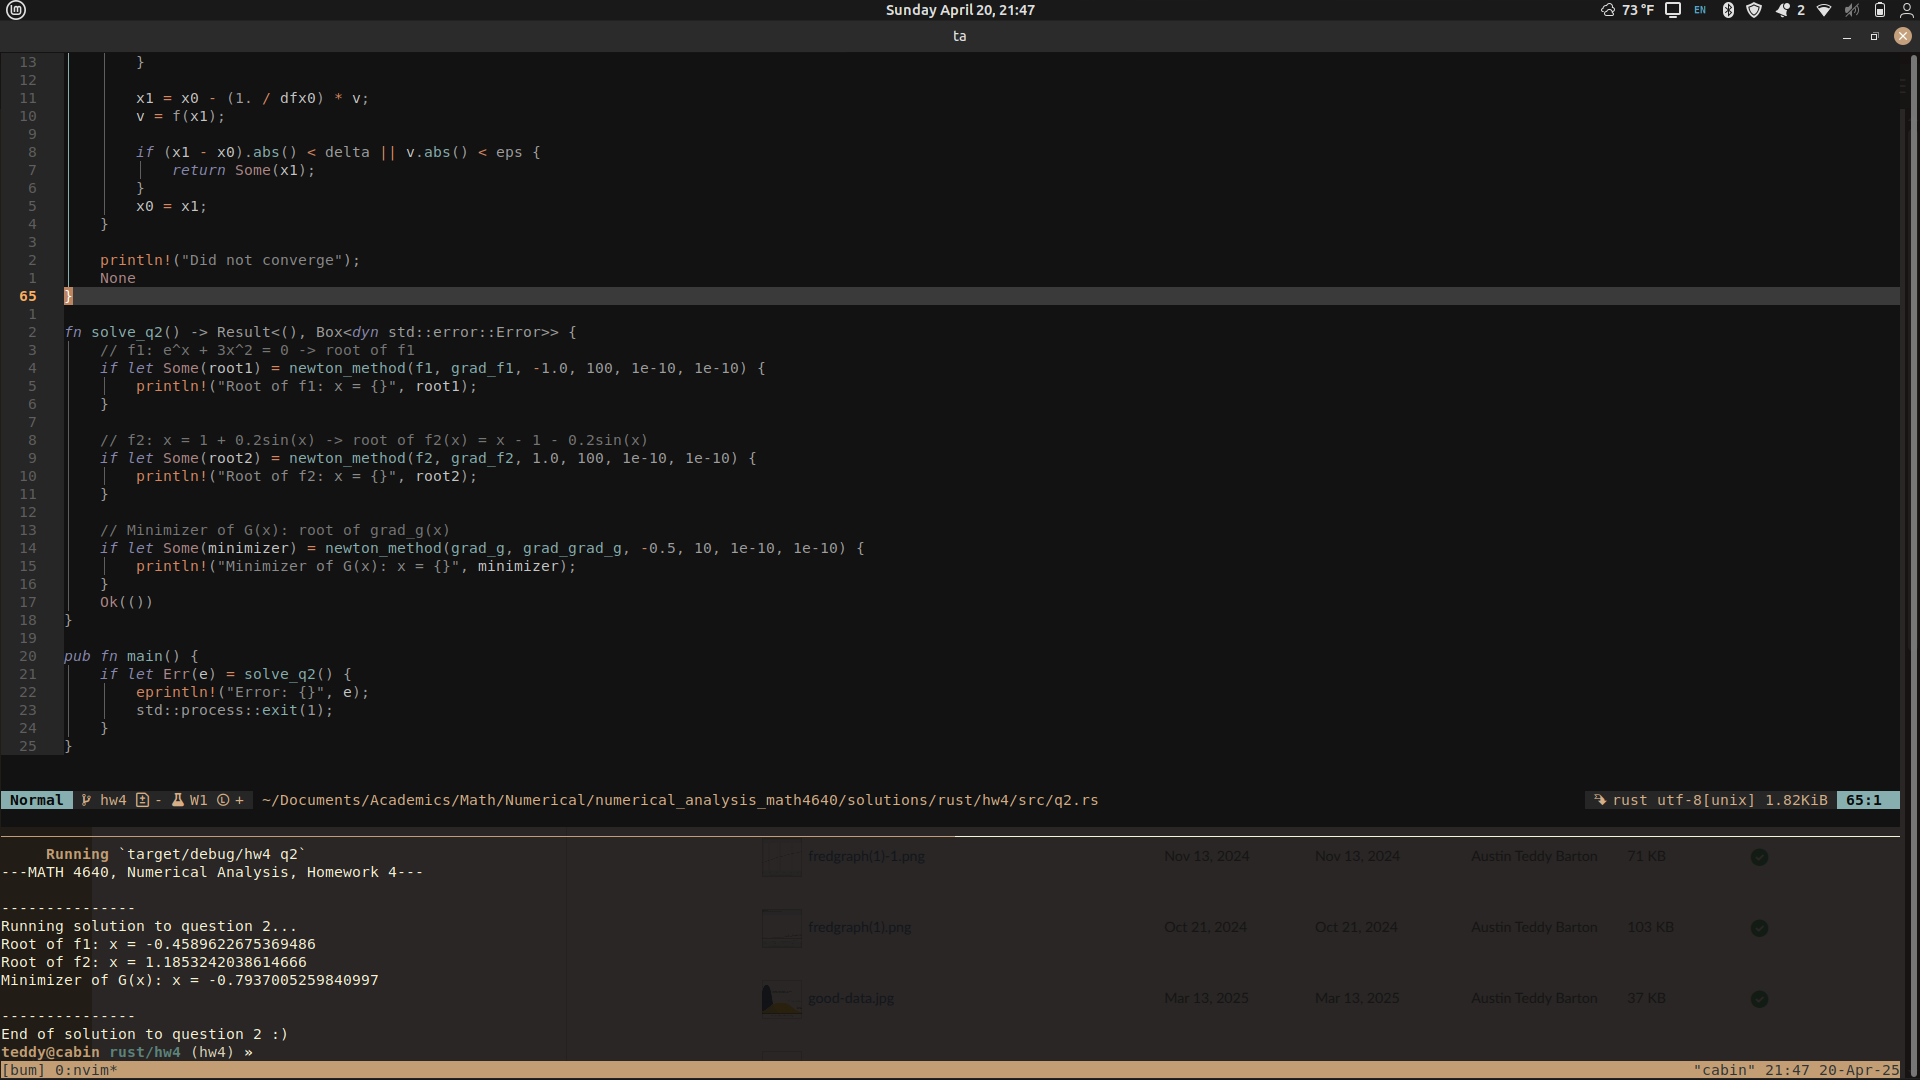
\includegraphics[width=0.8\textwidth]{numhw4q2-3.png}
\end{figure}

\clearpage

\hspace{18pt}\textbf{Problem 3:} \medskip
Please see attached PDF with all written solutions for questions 1-5 and 7-8.

\hspace{18pt}\textbf{Problem 4:} \medskip
Please see attached PDF with all written solutions for questions 1-5 and 7-8.

\hspace{18pt}\textbf{Problem 5:} \medskip
Please see attached PDF with all written solutions for questions 1-5 and 7-8.


\clearpage

\hspace{18pt}\textbf{Problem 6:} \medskip

With the code in the following screenshots are the outputs for the code.

\begin{figure}[!htbp]
	\centering
	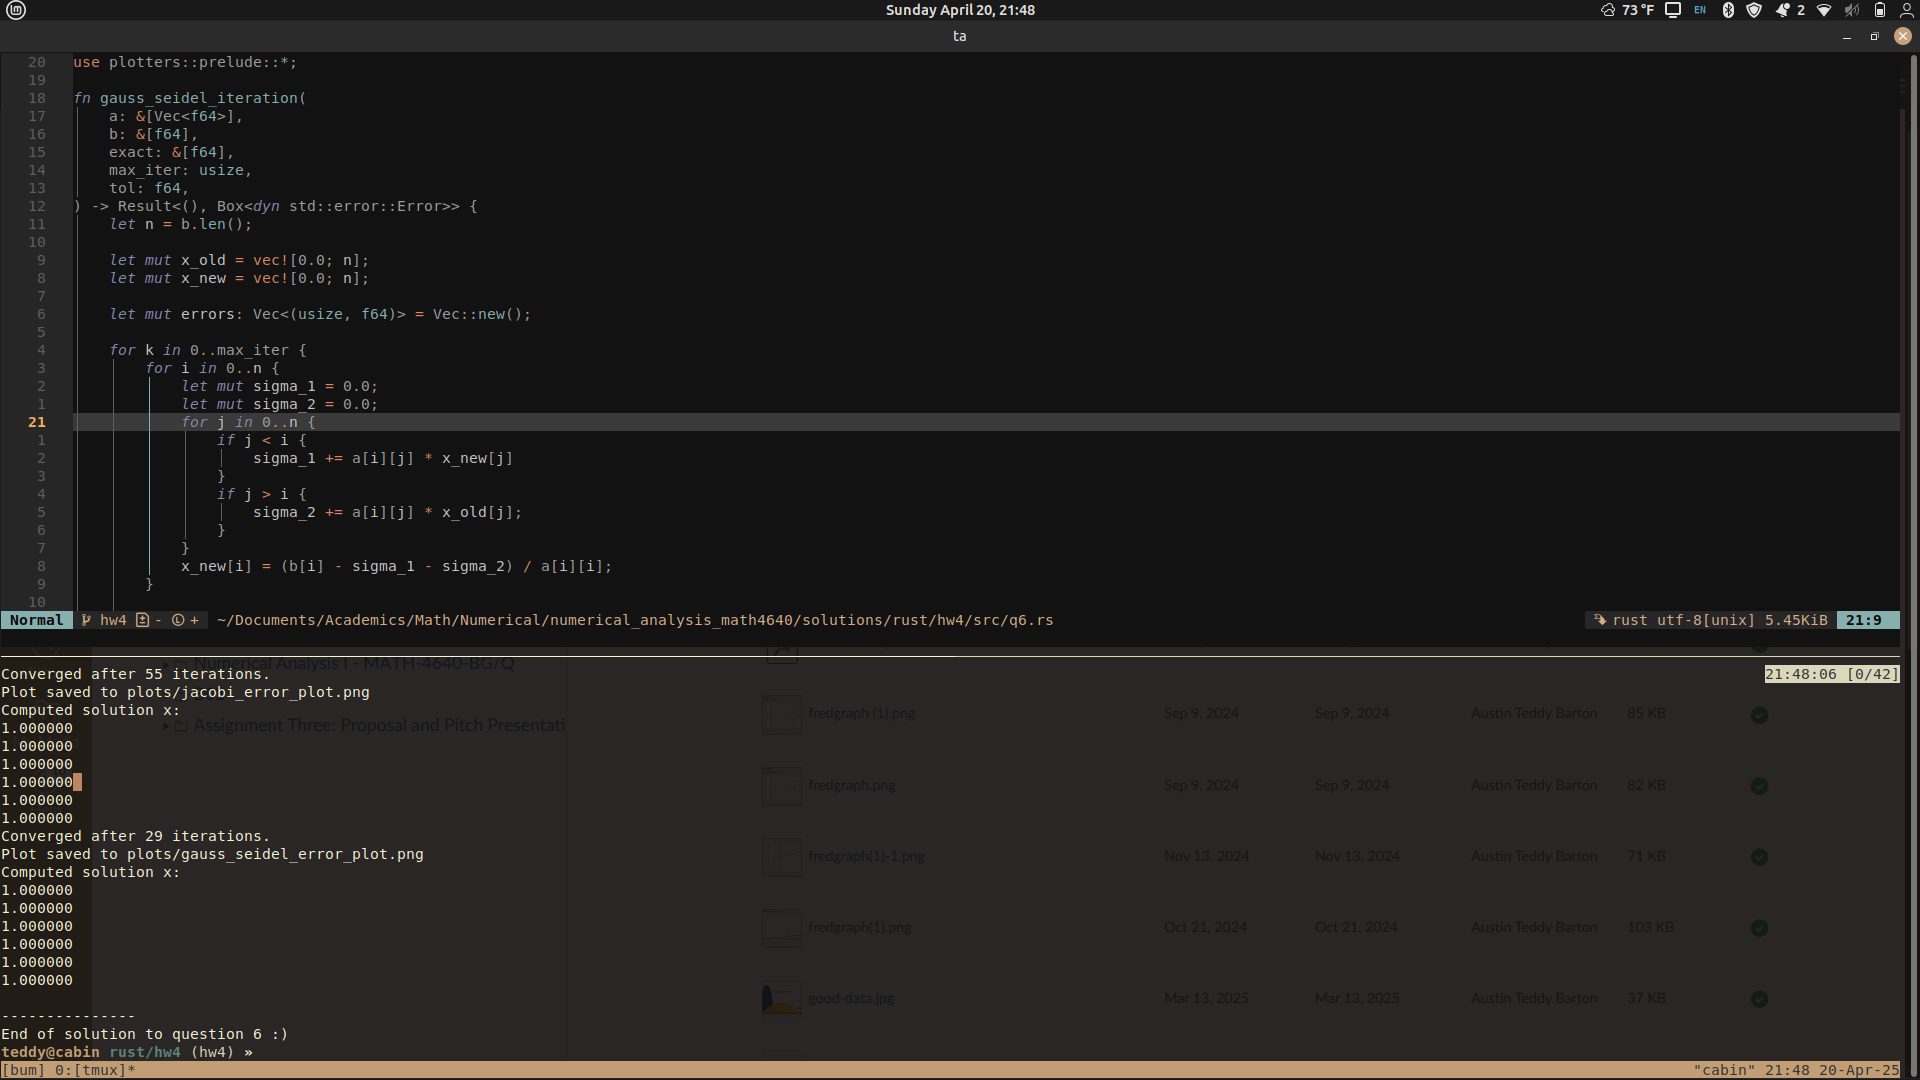
\includegraphics[width=0.8\textwidth]{numhw4q6-1.png}
\end{figure}
\begin{figure}[!htbp]
	\centering
	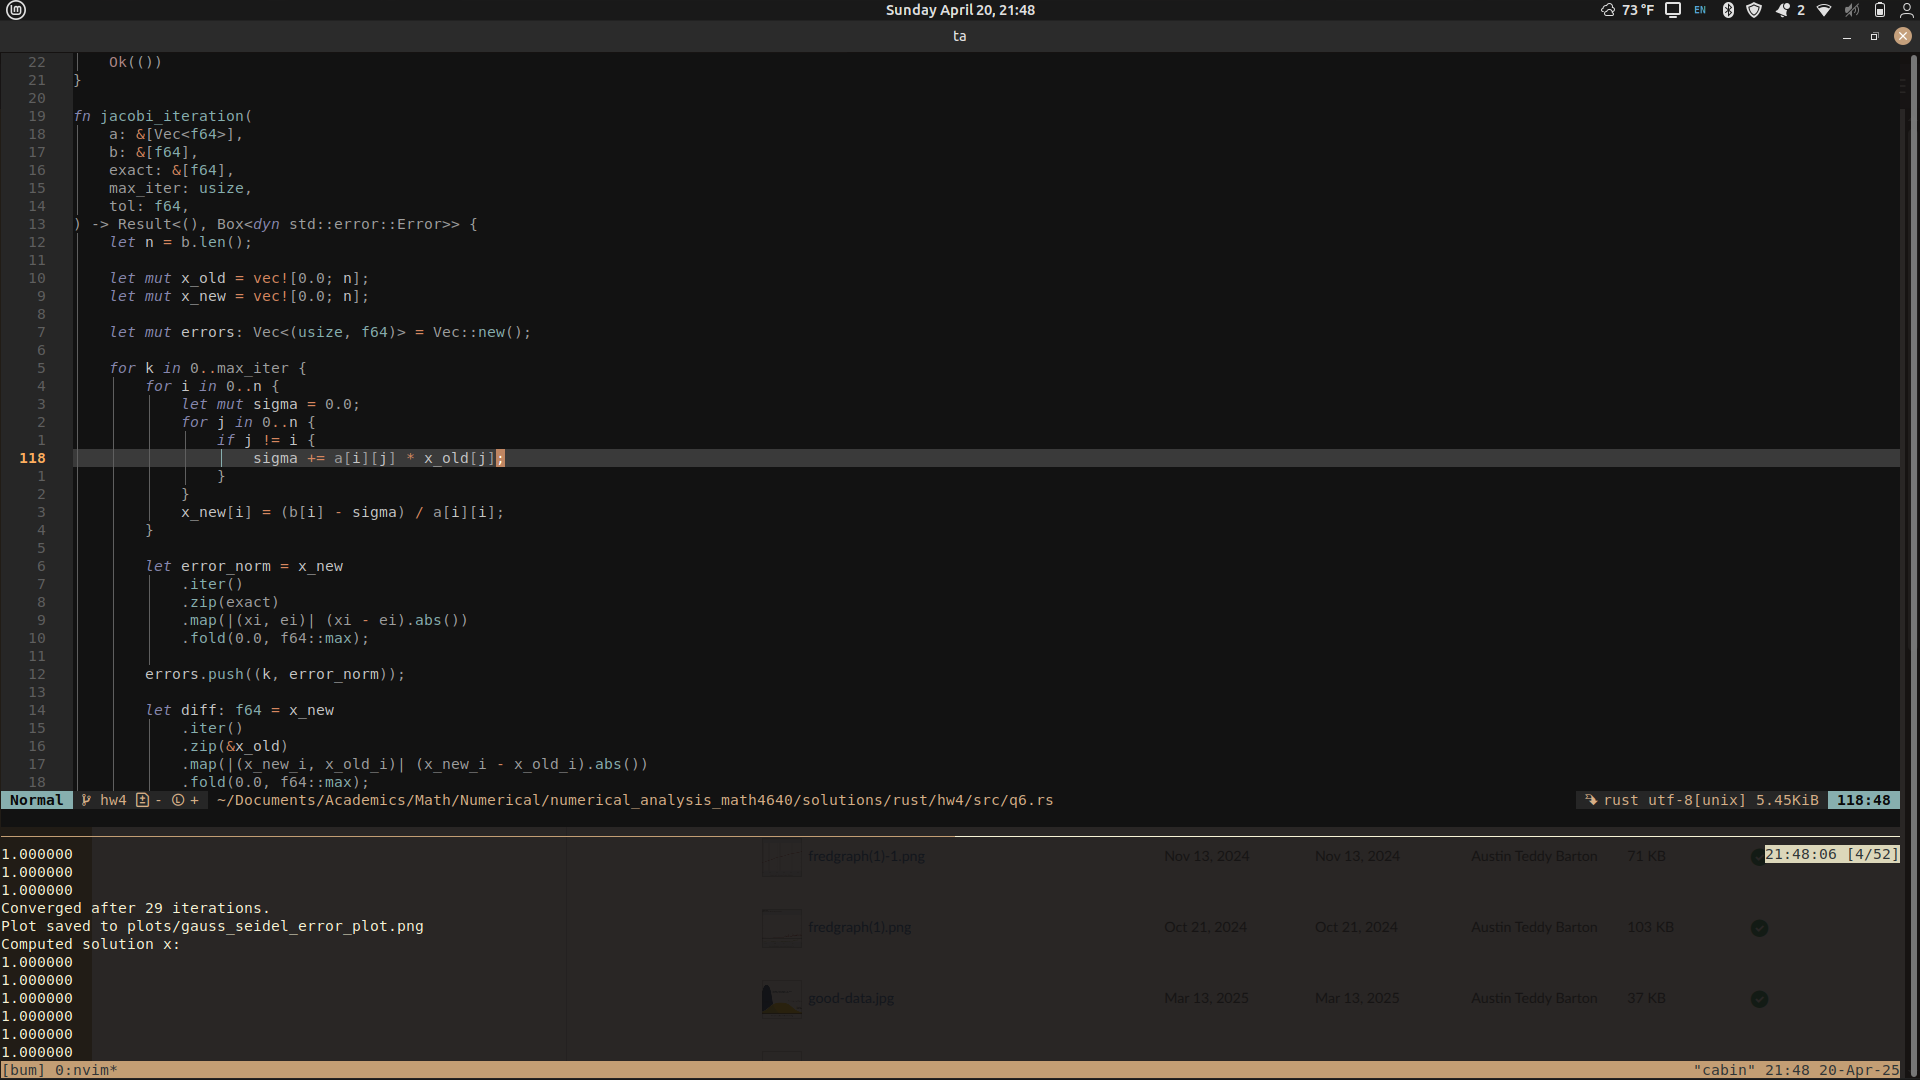
\includegraphics[width=0.8\textwidth]{numhw4q6-2.png}
\end{figure}
\begin{figure}[!htbp]
	\centering
	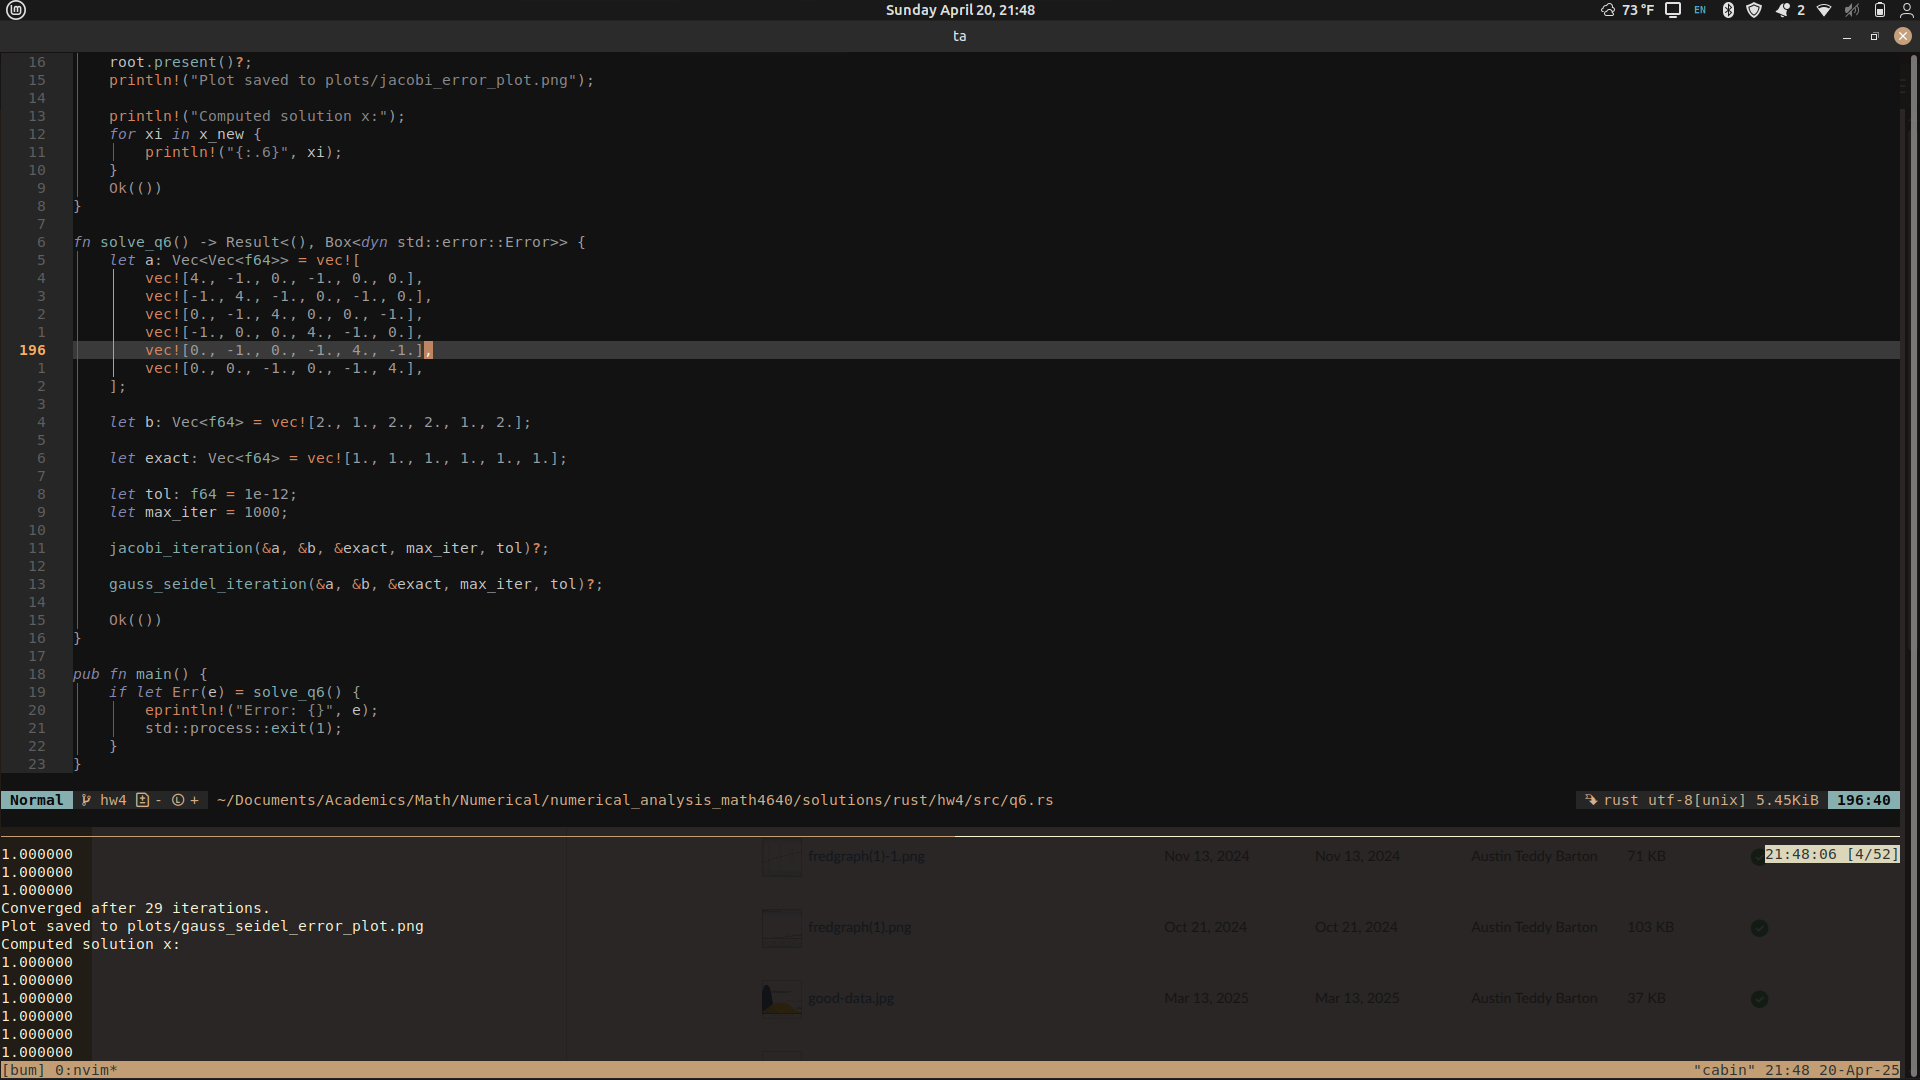
\includegraphics[width=0.8\textwidth]{numhw4q6-3.png}
\end{figure}
\begin{figure}[!htbp]
	\centering
	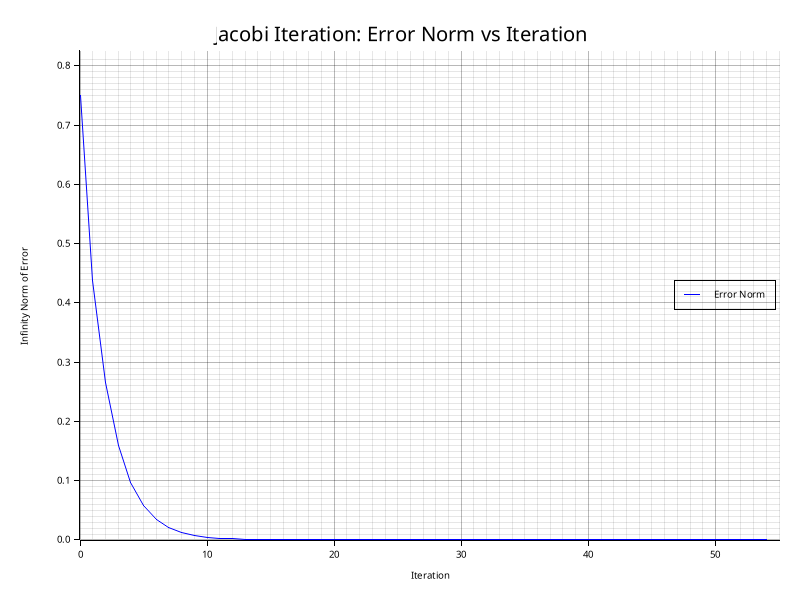
\includegraphics[width=0.8\textwidth]{jacobi_error_plot.png}
\end{figure}
\begin{figure}[!htbp]
	\centering
	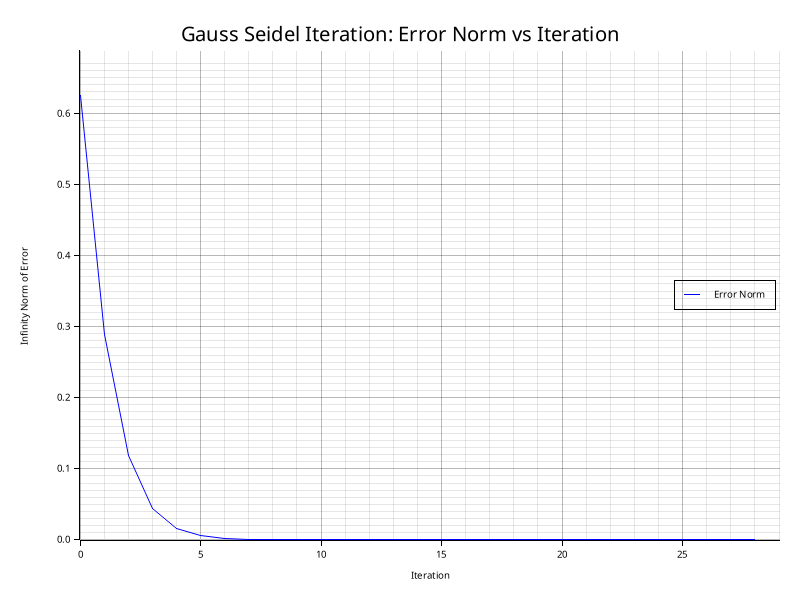
\includegraphics[width=0.8\textwidth]{gauss_seidel_error_plot.png}
\end{figure}

\clearpage

\hspace{18pt}\textbf{Problem 7:} \medskip
Please see attached PDF with all written solutions for questions 1-5 and 6-7.

\hspace{18pt}\textbf{Problem 8:} \medskip
Please see attached PDF with all written solutions for questions 1-5 and 7-8.

\clearpage

\section{Written Solutions}
\includepdf[pages=-, scale=0.85]{numhw4-solutions.pdf}

\end{document}
